\chapter{Computations and Readout}\label{sec:qubit-resonator}
To control and readout a superconducting qubit, it is coupled with feed lines coupling our control hardware to the quantum device. In this chapter, we will outline how the qubits are controlled, and how coupling a qubit to a resonator allows us to determine the state of the qubit by performing readout.


\section{Qubit Control}\label{sec:qubit_control}
When considering the qubit, a two level quantum mechanical system, where a state can be represented as a vector pointing on the Bloch sphere, Qubit control takes the form of rotating a vector to another point on the sphere. Even though, the state can be represented by just two parameters, namely the angles: zenith $\theta$ and azimuth $\phi$, three values are needed for an arbitrary rotation on the sphere.\footnote{Since a rotation consist of an axis (a vector represented by two angles $\theta, \phi$) and an angle, $\psi$, determining how much we rotate around that axis, we need in total the three values $\theta, \phi$ and $\psi$ to describe the arbitary rotation.}

\todo{Make sure this transition is coherent and makes sense}
The rotations on a Bloch sphere is a good analog for qubit rotations not only because it easy to visualize, but also because there is correspondence between the group of three dimensional rotation, $SO(3)$ and unitary evolution on a two level system, $SU(2)$. This correspondence also gives names to many of the operators in ... 

To fully control the two level qubit system, we need a \textit{Universal Gate Set}, from which every other rotation/unitary transformation can be build from. A very common one is the pauli gate set consisting of $\{\identity, X, Y, Z\}$ namely the identity and X, Y, Z gates defined by the pauli matrices:
\begin{fullwidth}
\begin{equation}
    \identity = \begin{pmatrix}
        1 & 0 \\ 
        0 & 1
    \end{pmatrix}, \quad
    X = \begin{pmatrix}
        0 & 1 \\ 
        1 & 0
    \end{pmatrix}, \quad
    Y = i\begin{pmatrix}
        0 & -1 \\ 
        1 & 0
    \end{pmatrix}, \quad
    Z = \begin{pmatrix}
        1 & 0 \\ 
        0 & -1
    \end{pmatrix}, \quad
\end{equation}
\end{fullwidth}
these gates are also considered the generators of the gates, since the rotations are made by exponiation of the gates, for example a $\pi/2$ rotation around the $X$-axis is made by: \todo{Write out as matrix}
\begin{equation}
    R_X^{\pi/2} = e^{i \frac{\pi}{2} \hat{X}}    
\end{equation}
When comparing this to the time evolution described in section \ref{sec: Time Evolution}, the gates correspond to the Hamiltonian and by applying the gate a certain amount of time, we can adjust the angle of the rotation. To completely control a qubit, the goal is now clearer: we need the ability to apply a full gate set to a qubit, which can be done by adding terms to the Hamiltnonian. 
\todo{I think, I want to do a bit more in this section. Just read it through and see if we want more group-theoretical way of thinking and how to integrate it better.}

If we were to further extend the scope to multi qubit gates, we would also need one fully-entangling two qubit gate to have complete the Universal Gate Set. Most commonly, this would be the Control-Not or a Control-phase gate. \cite{krantz_quantum_2019} \todo{add one more source maybe?}


\subsection{Capacitative Coupling}
By running a voltage line to the qubit and coupling it capacitatively, we can add an element $\propto \hat{n}V(t)$ to the Hamiltonian, where the factors are given by the capacitance of the device and the capacitor coupling them. \todo{This part may not be totally clear for a transmon} If we were to consider the charge matrix in the energy basis of the LC-basis (harmonic oscillator), it can be decomposed into $\hat{n} \propto -i(a - a^\dagger)$ coupling the different energy levels. While the transmon Hamiltonian differs a bit from the LC-circuit it is a good approximation, especially for the lower energy levels, so we write it simply $\hat{n} \propto -i (\sigma_- - \sigma_+)$ where we are restricted the space to just the computational basis.

By applying a voltage, we thus get a contribution to the Hamiltonian of the form:
\begin{equation}
    H_{QD} = - \Omega(t) i \left(\sigma_+ - \sigma_- \right) = \Omega(t) \hat{Y}
\end{equation}
Where $\Omega(t)$ consist of our controlled voltage along with a scaling dependent on the coupling to qubit.  

\paragraph{Note} - This is a bit of an approximation and to get the proper qubit behaviour, we would need to calculate the $n_{ij} = \mel{i}{\hat{n}}{j}$ matrix in the energy eigenbasis. In all our setups, the diagonal will however still be neglible, so the next argument should still hold \todo{Is there a better argument than simply $\approx$ Harmonic Oscillator?}

\subsection{The Qubit in the Interaction Picture}
With a qubit in its energy eigenbasis truncated to its computaional basis the Hamiltonian can be written in the following form:
\begin{equation}
    H = \frac{1}{2} \hbar \omega_{q} \sigma_z
\end{equation}
where the $\omega_q = \omega_{01} = (E_1 - E_0) / \hbar$. And adding the control from the voltage described above, we find:
\begin{equation}
    H = \frac{1}{2} \hbar \omega_{q} \sigma_z + \Omega V(t) \sigma_y
\end{equation} \todo{Non consistent notation}

We will now go into the interaction picture, where we consider $H_0 = \frac{1}{2} \hbar \omega_{q} \sigma_z$ and $H_d = \Omega V(t) \sigma_y$, such that the Hamiltnonian is simply $H = H_0 + H_d$. In the interaction frame, we go into a rotating reference frame, where
\begin{equation}
    \ket{\psi} \to \ket{\tilde{\psi}} = \mathcal{U}(t)\ket{\psi}, \quad \text{with}\quad \unitary(t) = e^{iH_0 t}
\end{equation}
In this basis, the Schrödinger equation becomes:
\begin{align*}
    i\partial_t \ket{\tilde{\psi}(t)} &= i \partial_t (\mathcal{U}(t) \ket{{\psi}(t)}) \\
    &= i \dot{\mathcal{U}}(t)\ket{\psi(t)} + i \mathcal{U}(t) {\ket{\Dot{{\psi}}(t)}}
\end{align*}
And using $\ket{\dot{\psi}(t)} = i H \ket{\psi}$ and $\ket{\psi(t)} = \mathcal{U}^\dagger(t) \ket{\tilde{\psi}(t)}$:
\begin{equation}
    i \partial_t \ket{\Tilde{\psi}(t)}= \left[(\dot{i \mathcal{U}}{(t)}\unitary^\dagger(t) + \unitary(t) H \unitary^\dagger(t)\right]\ket{\tilde{\psi}(t)}
\end{equation}
Such that the effective Hamiltonian in the rotating frame is given as:
\begin{equation}
    H_{eff} = \dot{i \mathcal{U}}{(t)}\unitary^\dagger(t)) + \unitary(t) H \unitary^\dagger(t)
\end{equation}
or in the case of the rotating frame of the qubit:
\begin{equation}
    H_{eff} = - H_0 + H_0 + \unitary(t) H_d \unitary^\dagger(t)
\end{equation}
where we have used that $\unitary^\dagger \unitary = \identity$ and that $\comm{\unitary}{H_0} = 0$. Substituting $H_D$ and $\unitary(t)$ we get \cite{krantz_quantum_2019}:
\todo{Set $\hbar = 1$ way before this points}
\marginnote[-2cm]{Writing $\sigma_y = i (\ket{1}\bra{0} - \ket{0}\bra{1})$ makes this calculation much easier.}
\begin{fullwidth}
\begin{align}
    H_{eff} &= \Omega V(t) i \exp\left(it\frac{\omega_q \sigma_z}{2}\right)  (\ket{1}\bra{0} - \ket{0}\bra{1} )\exp\left(-it\frac{\omega_q \sigma_z}{2}\right) \\
            &= \Omega V(t) i \left(e^{-it\omega_q}\ket{0}\bra{1} -  e^{+it\omega_q}\ket{1}\bra{0} \right) \\
            &= \Omega V(t) i \left((\cos(\omega_q t) - i\sin(\omega_q t))\ket{0}\bra{1} -  (\cos(\omega_q t) + i\sin(\omega_q t))\ket{1}\bra{0} \right) \\
            &= \Omega V(t) \left(\cos(\omega_q t)\sigma_y - \sin(\omega_q t) \sigma_x \right)
\end{align}
\end{fullwidth}
Where we see that in the rotating frame, we find both $\sigma_x$ and a $\sigma_y$ in the hamiltonian.

\subsection{X, Y and virtual Z}\label{sec:how_to_make_gates}
To arrive at the gates, we choose a pulse in the voltage line of the form:
\begin{equation}
    V(t) = s(t) (\sin(\omega_d t + \phi))
\end{equation}
where $s(t)$ is the envelope of our pulse with driving frequency $\omega_d$ and phase shift $\phi$. Defining $I = \cos(\phi), Q = \sin(\phi)$, we can write the pulse as:
\begin{equation}
    V(t) = s(t) \left(I \cos(\omega_d t) + Q \sin(\omega_d t)\right) 
\end{equation}
Such that the effective driving hamiltonian gives:
\begin{equation}
    H_{eff} = \Omega s(t) \left(I \cos(\omega_d t) + Q \sin(\omega_d t)\right)   \left(\cos(\omega_q t)\sigma_y - \sin(\omega_q t) \sigma_x \right)
\end{equation}


\paragraph{Rotating Wave Approximation} We will now perform the infamous rotating wave approximation (RWA). The basic concept is to decompose our Hamiltonian into fast and slow oscillating terms. If we have a Hamiltonian $H = H_{slow}(t) + H_{fast}(t)$, the time evolution operator becomes\footnote{Here we assume that the hamiltonian commutes with itself at different times, which is the case for the one we are dealing with} $\unitary(t) = \exp(i\int_0^tdt'H_{slow}(t') + i\int_0^tdt'H_{fast}(t'))$, but at any oscillation rate were the slow oscillating term gives a non-vanishing value, the fast oscillating term will cancel in the integral. We thus get $\unitary(t) \approx \exp(i\int_0^tdt'H_{slow}(t'))$ and for relevant dynamics, we can just consider $H\approx H_{slow}(t)$. \todo{Tighten this section, it is because it averages, maybe also check the footnote with Sakurai}

Rewriting the Hamiltonian with the product to sum trigonometric identities\footnote{An example is the $\cos(\alpha)\cos(\beta)=\frac{1}{2}(\cos(\alpha-\beta) + \cos(\alpha + \beta))$}, one would get: 

\begin{fullwidth}
    
\begin{align}
H_{eff} &= \Omega s(t) \left((I \cos(\omega_d t) + Q \sin(\omega_d t)) \cdot \cos(\omega_q t)\sigma_y - \left(I \cos(\omega_d t) + Q \sin(\omega_d t)\right) \cdot \sin(\omega_q t) \sigma_x \right) \\
H_{eff} &\approx \Omega s(t) \left((-I \cos(\delta t) + Q \sin(\delta t))\sigma_y + \left(I \cos(\delta t) - Q \sin(\delta t)\right) \sigma_x \right)
\end{align}
\end{fullwidth}\todo{How does this look with $\delta = 0$, how do we choose the time and envelope to make a specific gate.}
where $\delta = \omega_q - \omega_d$ and we applied the RWA in the second line to eliminate oscillating terms of frequency $\omega_q + \omega_d \gg \omega_q - \omega_d$. 

Since our driving hardware allows us control of $\phi$ and thus $I, Q$ as well as the driving frequency, we can add an x-gate by having $I = 1, Q = 0$ while driving on the qubit frequency, such that $\delta = 0$. The $y$-gate is done exactly the same, but at a $\pi/2$ rotation, such that $I = 0, Q = 1$. 
To complete our 1-qubit universal gate set, we now just lack the $\sigma_z$ gate. Since $\sigma_y$ and $\sigma_x$ pulses are defined in a rotating frame, we can just virtually rotate the phases to make a "virtual" z-gate. Thus a z-gate is not made by applying a gate, but by simply moving our reference frame, and corresponds to us rotating $I$ and $Q$ into each other. \cite{krantz_quantum_2019}

\begin{marginfigure}[-5 cm]
    \centering
    \missingfigure{Illustration of Virtual Z }
    \caption{Caption}
    \label{fig:control_virtual_z}
\end{marginfigure}


\section{Coupling to a Resonator}\todo{Need citation}
\todo{This section is based on \cite{boissonneault_dispersive_2009} and \cite{boissonneault_improved_2010}}  
In order to readout the qubit, without altering its state, we couple it do a resonator that is gonna work as a probe. While we use a resonator, because of its harmonic oscillator nature, we could also use a cavity and let our qubit interact with standing waves here. The physics is also more or less the same as in cavity QED, but being able to make a resonator..

In section \ref{sec:forming_qubits}, we described how having an LC circuit in superconducting materials give rise to a quantum harmonic oscillator with Hamiltonian:
\begin{equation}
    H_r = \omega_r \; a^\dagger a
\end{equation}
The resonator can now be coupled to the transmon by connecting them with a capacitor. This gives a $C_g V_r V_t$ potential. Using that $V_{r/t} = 2e n_{t/r} / C_{t/r}$ the potential can be written as $4e^2C_g  n_t n_r / C_r C_t$ or by simply defining the coefficient as $g$, the coupling is given by:
\begin{marginfigure}
    \centering
    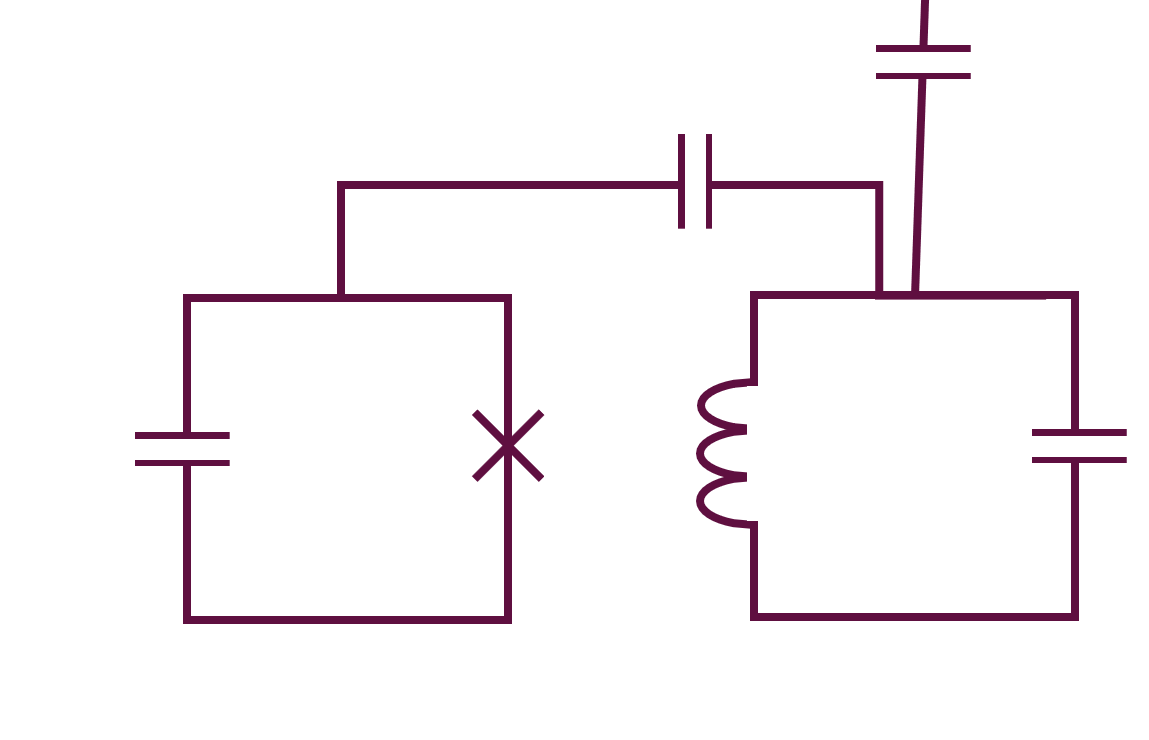
\includegraphics{Figs/Sections/computations_and_readout/qubit_resonator_feedline.png}
    \caption{A schematic of a Transmon coupled capacitatively to a resonator, which again is coupled to a feed line.}
    \label{fig:schematic_qubit_res}
\end{marginfigure}
\begin{equation}
    H_{int} = g n_c n_r 
\end{equation}
By using that $n_c \propto a + a^\dagger$ and $n_t \propto \sigma_+ + \sigma_-$ we obtain the Jaymes Cunning interaction:
\begin{equation}
    H_{int} = g (a + a^\dagger) (\sigma_- + \sigma_+)
\end{equation}
Where the proportions are absorbed into the coupling strength $g$. 


\subsection{Rotating Wave Approximation} \todo{Need citation}
To optimize the computation time, it is beneficial to get rid of fast oscillating terms. First we choose to go into the interaction picture, where we try to cancel the time evolution of the non-interacting Hamiltonian.
\begin{equation}
    H_0 = \omega_r \; a^\dagger a + \omega_t\frac{\sigma_z}{2} 
\end{equation}
where the associated time evolution operator will be:
\begin{equation}
    U_0(t) = e^{-iH_0t}
\end{equation}
In the interaction picture, we will now have: $\ket{\psi} \rightarrow U^\dagger(t)\ket{\psi}$ to counteract the fast oscillations from the $H_0$ term. The Hamiltonian will transform as: $H \rightarrow U^\dagger(t) H \; U(t)$. This yields a Hamiltonian given by:
\begin{align*}
    H_{int}(t) = H_0 + g \left(e^{it(-\omega_r - \omega_t)} a \sigma_- + e^{it(\omega_r - \omega_t)} a^\dagger \sigma_-\right.  \\ 
    \left.e^{it(-\omega_r + \omega_t)} a \sigma_+ + e^{it(\omega_r + \omega_t)} a^\dagger \sigma_+\right)
\end{align*}
We now perform the rotating wave approximation, where we drop fast oscillating terms:\marginnote{This works as the time-evolution operator is given by $U = \exp(i\int dt H)$ so fast oscillating term will cancel if the time interval is sufficiently large.}
\begin{equation}
    H_{int}(t) = H_0 + g \left(e^{it\Delta}a^\dagger\sigma_- +  e^{-it\Delta}a\sigma_+\right)
\end{equation}
where $\Delta = \omega_r - \omega_t$ is the detuning between the resonator and the transmon. Back in the Schödinger picture, we can simply write:
\begin{equation}
    H_{S} = H_0 + g \left(a^\dagger\sigma_- +  a\sigma_+\right)
\end{equation}

\subsection{Dispersive Regime}
We will now focus on the dispersive limit. Here the coupling is much smaller than the detuning between the resonator and transmon. We introduce the parameter:
\begin{equation}
    \lambda = \frac{g}{\Delta} \ll 1
\end{equation}
% In this regime, the Jaynes-Cummings Hamiltonian can be diagonalized to first order $\lambda$ by applying the transformation:
% \begin{equation}
%     \boldsymbol{D} = \exp\left[\lambda (a^\dagger \sigma_- - a \sigma_+) \right]
% \end{equation}
% The Hamiltonian transforms as: 
% \marginnote{Using $e^{-\lambda X}He^{\lambda X} = H + \lambda \comm{H}{X} + \lambda^2 / 2! \comm{\comm{H}{X}}{X} \dots$}

% \begin{align*}
%     H &\rightarrow \boldsymbol{D}^\dagger H \boldsymbol{D} \\
%       &= \exp\left(-\lambda (a^\dagger \sigma_- - a \sigma_+) \right) H \exp\left(\lambda (a^\dagger \sigma_- - a \sigma_+) \right) \\
%       &= H + \lambda\comm{H}{(a^\dagger \sigma_- - a \sigma_+)} + \mathcal{O}(\lambda^2)
% \end{align*}
% Where we calculate the commutator as:
% \begin{fullwidth}
% \begin{align*}
%     &= \comm{H_0 + g(a^\dagger \sigma_- + a \sigma_+)}{(a^\dagger \sigma_- - a \sigma_+)} & \\
%     &= \comm{\omega_r \; a^\dagger a + \omega_t\frac{\sigma_z}{2} }{(a^\dagger \sigma_- - a \sigma_+)} + g \comm{(a^\dagger \sigma_- + a \sigma_+)}{(a^\dagger \sigma_- - a \sigma_+)} \\
%     &= \omega_r \left(a^\dagger a a^\dagger \sigma_- - a^\dagger a a \sigma_+ - a^\dagger a^\dagger a \sigma_- + a a^\dagger a \sigma_+ \right) \\
%     &= \omega_r \left(n a^\dagger \sigma_- - n a \sigma_+ - a^\dagger n \sigma_- + a n \sigma_+ \right)
% \end{align*}
% \end{fullwidth}
To obtain a form of the Hamiltonian, which is diagonal to first order in $\lambda$, we will use the \textit{Schrieffer Wolff transformation}. For a Hamiltonian of type $H = H_0 + \lambda V$, the idea is to apply a transformation of the type $\boldsymbol{D} = e^{\lambda S}$ to get: \footnote{Here we use, that the exponential of an operator is represented as its power series: $e^{\lambda S} = \sum_n (\lambda S)^n / n!$ and $e^{-\lambda  S} = \sum_n (-1)^n (\lambda S)^n / n!$}
\begin{align*}
    H' = \boldsymbol{D}^\dagger H \boldsymbol{D} &= e^{-\lambda S} (H_0 + \lambda V) e^{\lambda  S} \\
    &= H_0 + \lambda V + \comm{\lambda S}{H_0 + \lambda V} + \frac{1}{2!} \comm{S}{\comm{S}{H}} + \dots
\end{align*}
Now using $\lambda \ll 1$, we neglect terms of second order or higher in $\lambda$ and  diagonalize the Hamiltonian to first order if we choose $S$ such that $V + \comm{S}{H_0} = 0$. In our case, where a transmon is dressed by a resonator, we choose our transformation to be:
\begin{equation}
    S = (a \sigma_+ - a^\dagger \sigma_-)
\end{equation}
Such that:\footnote{Where we can use the commutator relation $\comm{AB}{C} = A\comm{B}{C} + \comm{A}{B}C$ to find $\comm{a^\dagger a}{a^\dagger} = a^\dagger$ and $\comm{a^\dagger a}{a} = - a$. While $\comm{\sigma_z}{\sigma_+} = -2\sigma_+$ and $\comm{\sigma_z}{\sigma_-} = 2\sigma_-$.}
\begin{align*}
    \comm{H_0}{S} &= \comm{\omega_r a^\dagger a + \omega_t \sigma_z / 2}{a \sigma_+ - a^\dagger \sigma_-} \\
    &= - \omega_r \left(a^\dagger \sigma_- + a \sigma_+\right) - \frac12 \omega_t \left(2a^\dagger \sigma_- + 2 a \sigma_+ \right) \\
    &= -  (\omega_r + \omega_t)\left(a^\dagger \sigma_- + a \sigma_+\right) = - \Delta \left(a^\dagger \sigma_- + a \sigma_+\right) \\
    &= - \frac{g}{\lambda} \left(a^\dagger \sigma_- + a \sigma_+\right) = - V 
\end{align*}\todo{Need a minus here... Make it clear that V is defined as $V\lambda, so V = \Delta I_-$. I think the minus is actually in the $\omega_t$}
Such that:
\begin{equation*}
    V + \comm{S}{H_0} = 0
\end{equation*}
While we get a new contribution to the Hamiltonian by:
\begin{align*}
    \comm{S}{V} &= \lambda g \comm{a^\dagger \sigma_- - a \sigma_+}{a^\dagger \sigma_- + a \sigma_+} \\
                &= \lambda g \left(a^\dagger a \sigma_- \sigma_+ - a a^\dagger \sigma_+ \sigma_-\right) \\
                &= 2 \lambda g \left(a^\dagger a \sigma_z + \frac12 \lambda g \sigma_+\sigma_-\right) \\
                &= \lambda^2 g^2 \ket{1}\bra{1} + 2 \chi a^\dagger a \sigma_z
\end{align*}
Where $\chi= g^2 / \Delta$ is the dispersive shift, which here is a measure of how much the resonator frequency moves depending on the state of the qubit, while the $\lambda^2 g^2 \ket{1}\bra{1}$ is a contribution to the first excited state of the qubit and will normally just be absorbed into a new qubit frequency. The full dispersive Hamiltonian now reads:

\begin{equation}
    H = \left(\Tilde{\omega}_r a^\dagger a + \chi a^\dagger a \right)  + \frac12 \Tilde{\omega}_{01} \sigma_z
\end{equation}

Where the qubit frequency is altered to include the shift from seeing the resonator.
\begin{marginfigure}
    \centering
    \missingfigure{Figure showing dispersive shift of two qubit states}
    \caption{Caption}
    \label{fig:dispersive_two_level_qubit}
\end{marginfigure}

\subsection{Generalization for Multi Level Qubit}
\todo{Cite the exercise by Sven, if that is possible, otherwise just ask where he has it from. Determine what to keep.}
In the above, we assumed that the qubit only have two states. In reality, this is not true, and we will have to consider multiple levels. As before we have energy for the resonator given by: $H_{res} = \omega_r a^\dagger a$ while the energy for an M-level qubit can be written generally as:
\begin{equation}
    H_{q} = \sum_{k = 0}^{M-1} \omega_k \ket{k}\bra{k}
\end{equation}
Where $\ket{k}$ is the k'th energy eigenstate of the qubit with corresponding energy of $\omega_k$. Allowing the M-level qubit to interact with the resonator by the Generalized Jaynes-Cumming model:
\begin{equation}
    H_1 =  \sum_{i,j} g_{ij} \ket{i}\bra{j} (a + a^\dagger ) 
\end{equation}
Where the jump strength $g_{ij}$ is related to the overlap of the eigenstates with the charge operator and the coupling energy ($g$): $g_{ij} = g \matrixel{i}{\hat{n}}{j}$. This gives the full Hamiltonian: 
% \begin{align}
%     H &= H_0 + H_1  \nonumber \\&= \omega_r a^\dagger a +  \sum_{k = 0}^{M-1} \omega_k \ket{k}\bra{k} + \sum_{i,j} g_{ij} \ket{i}\bra{j} (a + a^\dagger ) 
% \end{align}
\begin{fullwidth}
    \begin{equation}
        H = H_0 + H_1  = \omega_r a^\dagger a +  \sum_{k = 0}^{M-1} \omega_k \ket{k}\bra{k} + \sum_{i,j} g_{ij} \ket{i}\bra{j} (a + a^\dagger ) 
    \end{equation}
\end{fullwidth}
As in the two-level-system, we can make  use of the Schreiffer-Wolff transformation to diagonalize the Hamiltonian to second order in the perturbation variable. We want to apply the transfomration: \marginnote{\textbf{Probably remove $\eta$ here and just make the dispersive argument later}}
\begin{align}
    H' &= e^{S} H e^{-S} = H + \comm{S}{H} + \frac{1}{2}\comm{S}{\comm{S}{H}} + \dots \nonumber\\
                        &= H_0 + H_1 + \comm{S}{H_0 + H_1} + \frac{1}{2} \comm{S}{\comm{S}{H_0 + H_1}} + \dots
\end{align}
Where $S$ has to be an anti-hermitian operator to make this a unitary transformation. The goal is now to choose $S$ such that the linear terms in our perturbation disappear. This gives the condition $\comm{S}{H_0} = - H_1$. If we were to choose:
\begin{equation}
    S = \sum_{ij}g_{ij}\ket{i}\bra{j}\left(\frac{1}{\omega_{ij} - \omega_r}a + \frac{1}{\omega_{ij} + \omega_r} a^\dagger \right)
\end{equation}
with $\omega_{ij} = \omega_i - \omega_j$. The commutator gives:
\begin{fullwidth}
\begin{align*}
    \comm{S}{H_0} &= \sum_{ijk}g_{ij}\comm{\ket{i}\bra{j}\left(\frac{1}{\omega_{ij} - \omega_r}a + \frac{1}{\omega_{ij} + \omega_r} a^\dagger \right)}{\omega_r a^\dagger a + \omega_k \ket{k}\bra{k}} \\
    &= \sum_{ij} g_{ij}\ket{i}\bra{j} (\omega_j - \omega_i) \left(\frac{1}{\omega_{ij} - \omega_r}a + \frac{1}{\omega_{ij} + \omega_r} a^\dagger\right) \\
    &+ \sum_{ij} g_{ij} \ket{i}\bra{j} \omega_r \left(\frac{1}{\omega_{ij} - \omega_r} \comm{a}{a^\dagger a}  + \frac{1}{\omega_{ij} + \omega_r} \comm{a^\dagger}{a^\dagger a} \right) 
\end{align*}
\end{fullwidth}
And with $\comm{a^\dagger}{a^\dagger a} = - a^\dagger$ and $\comm{a^\dagger}{a a} = + a$. We obtain:
\begin{align*}
    &= \sum_{ij}g_{ij}\ket{i}\bra{j}\left(\frac{\omega_j - \omega_i - \omega_r}{\omega_{ij} + \omega_r} a + \frac{\omega_j - \omega_i - \omega_r}{\omega_{ij} + \omega_r} a^\dagger  \right) \\
    &= -\sum_{ij}g_{ij}\ket{i}\bra{j}(a + a^\dagger) = - H_1
\end{align*}
With this result, our transformed Hamiltonian now becomes:
\begin{align}
    H' &= H_0 + \comm{S}{H_1} + \frac12\comm{S}{\comm{S}{H_0 + H_1}} \dots \nonumber \\
       &= H_0 + \comm{S}{H_1} + \frac12\left( - \comm{S}{H_1} + \comm{S}{\comm{S}{H_1}}\right) \dots \\
       &= H_0 + \frac12\comm{S}{H_1} + \dots
\end{align}
In the dispersive limit, the coupling strength is much weaker than the detuning: $g_{ij} \ll w_{ij}$. Since S contains $g_{ij} / w_{ij}$ terms, we only go to the linear term in the dispersive approximation, and drop everything with higher orders of S. 

In this transformed basis, we find the "pertubation" entirely from: $H_{shift} = \frac12 \comm{S}{H_1}$ which can be calculated to:
\begin{fullwidth}
\begin{align*}
    2 H_{shift}&= \comm{\sum_{ij}g_{ij}\ket{i}\bra{j}\left(\frac{1}{\omega_{ij} - \omega_r}a + \frac{1}{\omega_{ij} + \omega_r} a^\dagger \right)}{\sum_{kl} g_{kl} \ket{k}\bra{l} (a + a^\dagger ) } \\
    &= \sum_{ijkl} g_{ij} g_{kl}\left[\ket{i}\delta_{jk}\bra{l}\left(\frac{1}{\omega_{ij} - \omega_r}a + \frac{1}{\omega_{ij} + \omega_r} a^\dagger \right)(a + a^\dagger)\right]\\
    &- \sum_{ijkl} g_{ij} g_{kl}\left[\ket{k} \delta_{li}\bra{j} (a + a^\dagger)\left(\frac{1}{\omega_{ij} - \omega_r}a + \frac{1}{\omega_{ij} + \omega_r} a^\dagger\right)\right]
\end{align*}
\end{fullwidth}
Going into the rotating frame terms proportional to $aa$ or $a^\dagger a^\dagger$ will be negligible since they are not energy conserving. Further, we only consider the diagonal elements of this matrix. Terms proportional to $\ket{i}\bra{i}$. We find: \todo{If we keep this, these calculations should be controlled.}
\begin{fullwidth}
\begin{align*}
    2 H_{shift} &= \sum_{ij} |g_{ij}|^2 \ket{i}\bra{i} \left[\frac{1}{\omega_{ij} - \omega_r}aa^\dagger - \frac{1}{\omega_{ji} + \omega_r} a^\dagger a + \frac{1}{\omega_{ij} - \omega_r}a^\dagger a - \frac{1}{\omega_{ji} + \omega_r}  a a^\dagger  \right]
\end{align*}
\end{fullwidth}

Using the commutation relation $\comm{a}{a^\dagger} = 1$, we can write it in the following form:
\begin{fullwidth}
\begin{equation}
    H_{shift} = \sum_{ij} \ket{i}\bra{i} |g_{ij}|^2 \left(\frac{1}{\omega_{ij} - \omega_r} + \left(\frac{1}{\omega_{ij} - \omega_r} + \frac{1}{\omega_{ij} + \omega_r} \right)a^\dagger a\right)
\end{equation}
\end{fullwidth}

And by defining the following quantities:
\begin{align}
    \chi_{ij} &= |g_{ij}|^2 \left(\frac{1}{\omega_{ij} - \omega_r} + \frac{1}{\omega_{ij} + \omega_r} \right) \\
    \delta_{ij} &= \frac{|g_{ij}|^2 }{\omega_{ij} - \omega_r} \\
    \chi_{i} &= \sum_j \chi_{ij} \\
    \delta_{i} &= \sum_j \delta_{ij} 
\end{align}
The dispersive m-level qubit and resonator system can be written as:
\begin{equation}
    H' = \omega_r a^\dagger a + \sum_k \omega_k \ket{k}\bra{k} + \sum_{kl}\ket{k}\bra{k}(\delta_{kl} + \chi_{kl} a^\dagger a )
\end{equation}
Or in a more interpretable manner:
\begin{equation} \label{eq:multi_qubit_dispersive_hamiltonian}
    H' = \left(\omega_r + \sum_k \chi_k \ket{k}\bra{k} \right) a^\dagger a + \sum_k (\omega_k + \delta_k)\ket{k}\bra{k}
\end{equation}
This equation allows us to investigate the effect of the coupling between resonator and qubit. When coupled the qubit state shift the resonator frequency with $\chi_k$. While every qubit frequency is shifted slightly y $\delta_k$.

\begin{marginfigure}
    \centering
    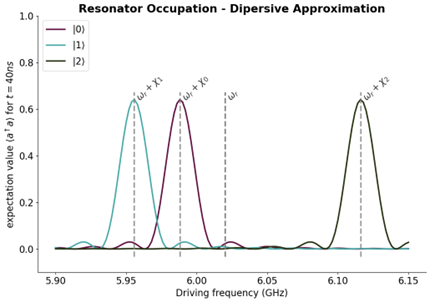
\includegraphics{Figs/Sections/computations_and_readout/three_qubit_states_dispersive.png}
    \caption{Driving the resonator will show resonance around a frequency determined by the qubit state. For a three state qubit the above is found:}
    \label{fig:three_state_dispersive}
\end{marginfigure}

Or by considering reducing the multi-level system to only the two lowest, we can write the equation in the simple form:
\begin{equation}\label{eq:two_level_qubit_dispersive}
    H = (\Tilde{\omega}_r + \chi \sigma_z) a^\dagger a + \frac12 \Tilde{\omega}_{01} \sigma_z
\end{equation}
where the shifts from the higher order terms have been absorbed into the new redefined frequencies. 



\subsection{Readout Drive in the Dispersive Approximation}
\todo{Currently this note is primarily how to enter the rotating frame of the drive. There should probably be more physics included. Transformation is taken from \cite{krantz_quantum_2019}}
When we perform a readout, we drive a capacitatively coupled line like we did in section \ref{sec:qubit_control}. Choosing a driving pulse with a rectangular envelope and phase 0, we have a contribution to the Hamiltonian of the form:
\begin{equation}
    H_{drive} = \epsilon\cos(\omega_d t)(a + a^\dagger) = \frac{\epsilon}{2} \left(e^{i\omega_d t} + e^{-i\omega_d t}\right)(a + a^\dagger)    
\end{equation}
where $\epsilon$ is the amplitude of the drive and $\omega_d$ is the drive frequency. Like already a few times before, we now want to enter the rotating frame to cancel rapidly oscillating terms. We choose the time dependent transformation:
\begin{equation}
    \unitary(t) = \exp\left(- i t \sum_k (\omega_k + \delta_k) \ket{k}\bra{k}\right) \otimes \exp \left(- i t \omega_d \;  a^\dagger a \right)
\end{equation}
To find effective Hamiltoninan:
\begin{equation}
    H_{eff} = \dot{i \mathcal{U}}{(t)}\unitary^\dagger(t)) + \unitary(t) H \unitary^\dagger(t)
\end{equation}
We find the contribution from the "centrifugal" term as:
\begin{equation}
    \dot{i \mathcal{U}}{(t)}\unitary^\dagger(t)) = - i t \sum_k (\omega_k + \delta_k) \ket{k}\bra{k} - it \omega_d \;  a^\dagger a
\end{equation}
The drive hamiltonian transforms as:
\begin{align*}
    H_{drive} &\to \unitary(t) H_{} \unitary^\dagger{t} \\
    &= \frac12 \epsilon (e^{i\omega_d t} + e^{-i\omega_d t}) \left[ \; \unitary(t)  (a + a^\dagger) \unitary^\dagger(t)\right] \\
    &= \frac12 \epsilon (e^{i\omega_d t} + e^{-i\omega_d t}) \left[ \;a e^{i \omega_d t} + a^\dagger e^{-i \omega_d t} \right]
\end{align*}
Neglecting the fast rotating terms ($\propto e^{\pm 2i\omega_dt}$), we get the effective drive Hamiltonian:
\begin{equation}
    H_{d, eff} = \epsilon(a + a^\dagger)
\end{equation}
Such that the total effictive Hamiltonian now becomes:
\begin{equation}
    H_{eff} =  \left(\omega_r - \omega_d + \sum_k \chi_k \ket{k}\bra{k}\right)a^\dagger a + \epsilon(a + a^\dagger)
\end{equation}
Which gives a nice time-independent Hamiltonian for m-level qubit which will prove ideal for simulation purposes. Here we chose to have a $\cos$ pulse with no phase, but we could (like in section \ref{sec:qubit_control}) have chosen a phase $\phi$, to get the last term as $\cos(\phi)\epsilon(a + a^\dagger) + \sin(\phi)i\epsilon(a - a^\dagger)$. Since this is only a matter of a phase, the actual form used may vary throughout the thesis. \todo{Would be nice with some figures/physics here. Maybe comment on the approximations.}



\section{I-Q Plane}
\todo{Check units and clean this a bit.}
To build up a visualization of the readout drive which later will be closely related to the measurements, we want to consider the phase plane of the resonator. As a start, lets consider the quantum harmonic oscillator subject to $H = \omega^2  x^2 + p^2$ with proper definitions of $x$ and $p$ which properly satisfy $\comm{x}{p} = i$. To diagonalize the Harmonic Oscillator, one usually introduces the raising and lowering operator by:
\begin{align}
    &a \propto x + ip \hfill &a^\dagger \propto x - ip \\
    &x \propto a + a^\dagger \hfill &p\propto i (a - a^\dagger)
\end{align}
Now, one can consider the harmonic oscillator either discretely in the $n = a^\dagger a$ eigenspace or in the continuous basis of $x$ and $p$. The same can be done with photons in a resonator. Where we consider the "quadratures" of the electric field, which we define as Q and I and are defined by the photon creation and annihilation operator in a way quite like the $x$ and $p$ operators of the harmonic oscillator \cite{knight}:
\begin{equation}
    Q = a + a^\dagger \hspace{2 cm} I = i(a^\dagger - a)
\end{equation}

\subsection{Coherent States}
When considering a Harmonic Oscillator, the number states have expectation values $\expval{x} = \expval{p} = 0$. To get non-zero values of these expectation values, one is required to have superposition states with adjacent components. Example: $c_n\ket{n} + c_{n+1} \ket{n+1}$, which would satisfy $\expval{x} \propto \expval{a + a^\dagger} \neq 0$. The more natural states would be eigenstates to the annihilation operator:
\begin{equation}
    a \ket{\alpha} = \alpha \ket{\alpha}
\end{equation}
Expanding $\ket{\alpha}$ in the Fock states gives us:
\begin{align}
    a \sum_n C_n \ket{n} = \alpha \sum_{n = 0} C_n \ket{n} \\
    \sum_{n = 1} C_n \sqrt{n} \ket{n - 1}
\end{align}
From where, we can compare the coefficients of the $\ket{n}$:
\begin{equation}
    \sqrt{n} C_n = \alpha C_{n - 1}
\end{equation}
Given $C_0$, we can now determine the rest of the series as:
\begin{equation}
    C_N = \frac{\alpha^n}{\sqrt{n!}} C_0 
\end{equation}
Such that $\ket{\alpha}$ can be found as: 
\begin{equation}
    \ket{\alpha} = C_0 \sum_n \frac{\alpha^n} {\sqrt{n!}} (a^\dagger)^n \ket{0} = C_0
\end{equation}
Where $C_0$ can be found from normalization as:
\begin{align}
    1 &= |C_0|^2 \bra{0}\sum_{n, m}\frac{(\alpha^*)^m} {\sqrt{m!}} a^m \frac{\alpha^n} {\sqrt{n!}} (a^\dagger)^n \ket{0} \\
    1 &= |C_0|^2 \sum_n \frac{|\alpha|^{2n} }{n!} = |C_0|^2 e^{|\alpha|^2} \\
    |C_0|^2 &= e^{-|\alpha|^2}
\end{align}
Which is satisfied by: $C_0 = e^{- |\alpha|^2 / 2}$. Thus a coherent state is given as:
\begin{equation}
    \ket{\alpha} = e^{-|\alpha|^2 / 2} \sum_n \frac{\alpha^n}{\sqrt{n!}} \ket{n}
\end{equation}
Where each complex $\alpha$ corresponds to a coherent state.

% \subsection{Overcompleteness / Properties of Coherent States}
% \textbf{This is probably relevant for the Q function} 

\subsection{Phase Space Representations}
\todo{This is a bit akward with the order since the density matrix is not presented before next section.} \noindent
When considering a way of representing a density matrix $\rho$ in phase space, we have the chance to define the properties we want. A natural way of thinking about this would be probability functions, which have certain properties. It would be useful to be able to express expectation values, $\expval{O} = \mel{\psi}{O}{\psi}$ in phase space. If we were to represent an operator in a coherent basis, it would take the form:
\begin{equation}
    O = \int d\alpha^2 O(\alpha, \alpha^*)\ket{\alpha}\bra{\alpha} 
\end{equation}
The expectation value $\expval{O}$ will now take the form: 
\begin{align*}
    \expval{O} &= \Tr{O \rho} \\
               &= \sum_n \bra{n} \int d\alpha^2 O(\alpha, \alpha^*)\ket{\alpha}\bra{\alpha} \rho \ket{n} \\
               &= \int d\alpha^2 O(\alpha, \alpha^*)\bra{\alpha} \rho \ket{\alpha}
\end{align*}
\marginnote[-1 cm]{Here we have used that $\mel{\alpha}{\rho}{n}$ is a scalar and commutes with the other operators while $\sum_n \ket{n}\bra{n} = \identity$.}
Here $\mel{\alpha}{\rho}{\alpha}$ takes the role of a probability distribution in the coherent phase space. To further ensure that the function is properly normalized, we demand the expectation value of the identity to equal 1:
\begin{align*}
    1 = \expval{\identity} &= \int d\alpha^2 \frac{1}{\pi} \mel{\alpha}{\rho}{\alpha}
\end{align*}
Such that we find the Husimi $Q$-function as:
\begin{equation}
    Q(\alpha) =  \frac{1}{\pi} \mel{\alpha}{\rho}{\alpha}
\end{equation}
which will serve as our probability distribution of a density matrix $\rho$ in the coherent phase space.

\subsection{Common States *}
Were we to solve the Hamiltonian in either the position or momentum basis, we would find that the ground state solution to be a Gaussian centered around the bottom of the square-potential and for higher states, we would have some multiplication with a Hermite Polynomial of corresponding order. This fact can be seen in figure \ref{fig:Q_func_examples} where the vacuum state is a 2D gaussian centered at the center (\textit{check validity of statement}). \\
Now for the higher Fock states ($n = 3$ is shown), we see a ring, which is centered with an average radius of $n$. A good intuition for this is the energy conservation of the harmonic oscillator. If we were to measure the position $x=0$ of a harmonic oscillator with non-zero energy, it would certainly have a non-zero momentum. Of course in quantum mechanics this is smeared a bit by Heisenberg Uncertainty Principle.\\
The coherent state described in the previous sections behaves like moving the vacuum around. The center of the distribution will be in $\alpha$.  

\begin{marginfigure}[-12 cm]
    \centering
    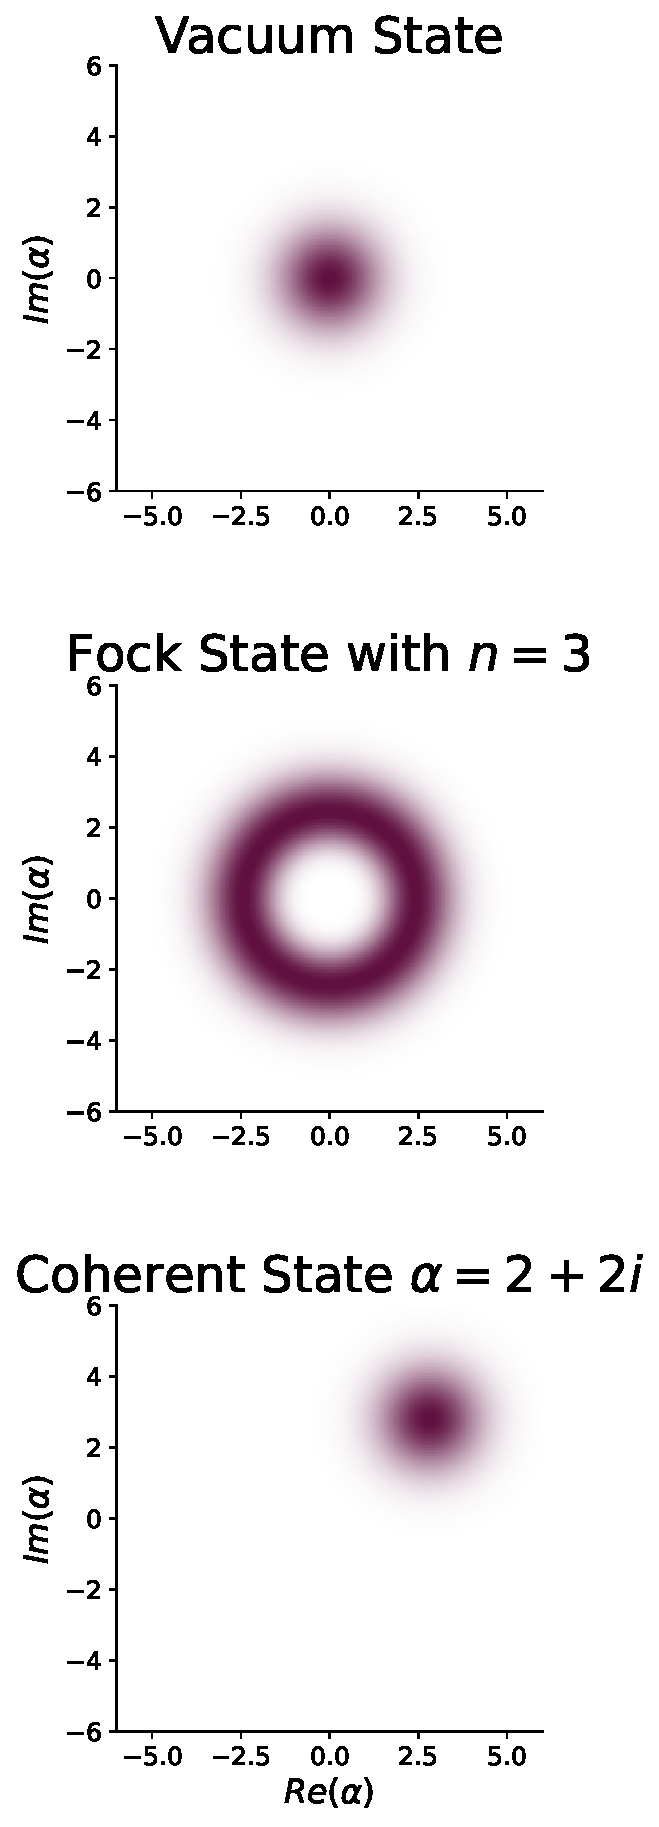
\includegraphics{Figs/Theory/Q_functions.pdf}
    \caption{Example of Different Q-functions for vacuum state, Fock state ($n = 3$) and a coherent state with $\alpha = 2 + 2i$.}
    \label{fig:Q_func_examples}
\end{marginfigure}

\subsection{The Driven Resonator in IQ Plane}\label{sec:driving_resonator_iq_plane}
With the new formulation of Q-functions we can visualize the readout drive as a separation in the IQ plane. Let us explore what happens, when we drive the resonator while considering the qubit to be a two level system subject to the Hamiltonian:
\begin{equation}
    H_{eff} =  \left(\omega_r - \omega_d + \chi \sigma_z\right)a^\dagger a + \epsilon(a + a^\dagger)
\end{equation}
If we were to take the time-derivative of the lowering operator of the resonator, we find:
\begin{equation}
    \dot{a}(t) = i\comm{H_{eff}}{a} = -i\comm{\left(\omega_r - \omega_d + \chi \sigma_z\right)a^\dagger a + \epsilon(a + a^\dagger)}{a}
\end{equation}
And using the commutation relatons, we find:
\begin{equation}
    \dot{a}(t) = -i \left(\left(\omega_r - \omega_d + \chi \sigma_z\right) a(t) + \epsilon\right)
\end{equation}
We now consider the resonator to be in a coherent state $\ket{\alpha}$ (initially we consider $\alpha(t=0) = 0$) and the qubit is in $\ket{k}$ with $k = 0,  1$. Applying our field operator from above, now gives us\todo{cite Blais}:
\begin{equation}
    \dot{\alpha}(t) \ket{\alpha(t), k} = - i \left(\left(\omega_r - \omega_d \pm \chi \right) \alpha(t) + \epsilon\right) \ket{\alpha(t), k} 
\end{equation}
\todo{Include figures. Does this calculation make sense before we add the dissipation?}


\begin{itemize}
    \item When driving the resonator, we move it in the IQ-plane
    \item What happens if we're slighly off resonant. We see a curve
    \item Display the path of two qubit when we apply a drive inbetween the resonances. 
\end{itemize}


% \vspace{1 cm}
% We now want to enter the rotating frame of the resonator. To make sure we also cancel the fast oscillating terms of the qubit, we choose to do the time-dependent transformation:
% \begin{equation}
%     \ket{\psi} \to \ket{\tilde{\psi}} = \mathcal{U}(t)\ket{\psi}
% \end{equation}
% In this basis, the Schrödinger equation becomes:
% \begin{align*}
%     i\partial_t \ket{\tilde{\psi}(t)} &= i \partial_t (\mathcal{U}(t) \ket{{\psi}(t)}) \\
%     &= i \dot{\mathcal{U}}(t)\ket{\psi(t)} + i \mathcal{U}(t) {\ket{\Dot{{\psi}}(t)}}
% \end{align*}
% And using $\ket{\dot{\psi}(t)} = i H \ket{\psi}$ and $\ket{\psi(t)} = \mathcal{U}^\dagger(t) \ket{\tilde{\psi}(t)}$:
% \begin{equation}
%     i \partial_t \ket{\Tilde{\psi}(t)}= \left[(\dot{i \mathcal{U}}{(t)}\unitary^\dagger(t) + \unitary(t) H \unitary^\dagger(t)\right]\ket{\tilde{\psi}(t)}
% \end{equation}
% Such that the effective Hamiltonian in the rotating frame is given as:
% It is now possible, to use this fact to simultaneously remove the time-dependence from the drive and remove the fast oscillating terms from the Qubit states. We now want to transform the resonator driving hamiltonian and the dispersive hamiltonian from Eq. \ref{eq:multi_qubit_dispersive_hamiltonian}. We choose: 
% Such that the effective Hamiltonian from the system gets the "centrifugal" contribution:
% While the Hamiltonian stays constant, since $\comm{H_{sys}}{\unitary(t)} = 0$:
% \begin{equation}
%     \unitary(t) \; H_{sys} \; \unitary^\dagger(t) = H_{sys}
% \end{equation}